
\chapter{Conceitos} \label{conceitos}


Neste capítulo, abordam-se os conceitos fundamentais da interação da luz com os materiais na computação gráfica. Destaca-se a importância da reflexão da luz, explorando as BRDFs e modelos comuns. Além disso, são discutidos elementos-chave na criação de compiladores e no processo de \textit{shading} na GPU.


Especificamente na \autoref{radiometria}, são apresentados os conceitos fundamentais relacionados à luz, como a capacidade de um material refletir raios de luz e sua importância na computação gráfica e renderização. Destaca-se a relação entre a intensidade de um pixel de imagem, a iluminação, a orientação da superfície e a definição de funções de refletância, as BRDFs. Já na \autoref{brdfmodels}, são destacados alguns modelos comuns de BRDFs.


A \autoref{shading} aborda o processo de \textit{shading} e o funcionamento do \textit{pipeline} de renderização na GPU. Nela, são introduzidos os processos de transformação de vértices e de determinação da cor dos fragmentos, mostrando exemplos de código. 


Na \autoref{compiladores}, é fornecida uma visão abrangente dos elementos essenciais na criação de compiladores. Ela começa com a definição de conceitos fundamentais, como cadeias de símbolos e alfabetos, necessários para entender linguagens formais. Além disso, é discutida a importância das gramáticas na definição de linguagens e é descrito o processo de compilação, incluindo a análise léxica, a análise sintática, o Pratt \textit{Parsing} e análise semântica.






\section{Radiometria} \label{radiometria}


A radiometria trata de conceitos fundamentais relacionados à luz. Ela abrange a capacidade de um material de superfície receber raios de luz de uma direção e refleti-los em outra 
\cite{radiometry_introduction}. No contexto da computação gráfica, a radiometria desempenha um papel crucial na compreensão do comportamento da luz em uma cena.


Na renderização, a intensidade de um pixel da imagem depende de vários fatores, como iluminação, orientação e refletância da superfície. A orientação da superfície é determinada pelo vetor normal em um dado ponto, enquanto a refletância da superfície diz respeito às propriedades materiais da mesma.


Para compreender e interpretar a intensidade de um pixel em uma imagem, é essencial compreender os conceitos radiométricos. A radiometria quantifica o brilho de uma fonte de luz, a iluminação de uma superfície, a radiância de uma cena e a refletância da superfície.


Renderizar uma imagem envolve mais do que capturar cor \cite{radiometry_color}; requer conhecimento da intensidade de luz em cada ponto da imagem, isto é, a quantidade de luz incidente na cena que alcança a câmera. A radiometria ajuda na criação de sistemas e unidades para quantificar a radiação eletromagnética, considerando um modelo simplificado no qual a luz é tratada como fótons que viajam em linha reta. 


\subsection{Energia Radiante e Fluxo} \label{fluxo}


Vários processos físicos convertem energia em fótons, como radiação de corpo negro e fusão nuclear em estrelas \cite{black_body_radiation}. Quantificar a energia radiante total de uma cena é necessário para quantificar o brilho da imagem, que envolve entender a energia dos fótons colidindo com objetos \cite{rendering_judice}.


A \autoref{eq-radiant-energy} expressa a energia radiante \( Q \) \cite{pbr}, que considera a energia total de todos os fótons atingindo a cena durante toda a duração, onde:  \( c  \approx 3,00 \times 10^8 \) m/s (metros por segundo) é a velocidade da luz; \( \lambda \) representa o comprimento de onda, uma variável que abrange o espectro visível, aproximadamente entre \( 389 \times 10^{-3} \)m e \(700 \times 10^{-3} \)m; \( h \) denota a constante de Planck, aproximadamente \( 6,626 \times 10^{-34} \) J$\cdot$s (joule-segundo).




\begin{equation}\label{eq-radiant-energy}
Q = \frac{hc}{\lambda}
\end{equation}






É interessante observar a evolução da energia radiante ($Q$) ao longo do tempo. Isso dá origem ao conceito de fluxo radiante $\phi$, que é medido em impactos de cada fóton por segundo em uma superfície. Sua unidade é joules por segundo e está representada na \autoref{eq-fluxo-radiante}.



\begin{equation} \label{eq-fluxo-radiante}
  \phi = \frac{dQ}{dt} \left[\text{J/s}\right] 
\end{equation}


A irradiância quantifica o número de impactos dos fótons em uma superfície por segundo por unidade de área. Mais precisamente, podemos definir a irradiância $E$ ao considerar o limite do fluxo radiante $\phi$ diferencial por área $A$ diferencial em um ponto $p$ \cite[~5.4.1]{pbr}. Assim, temos uma métrica mais específica para renderizar imagens com precisão. Sua fórmula é demonstrada na \autoref{eq-irradiance}.


\begin{equation} \label{eq-irradiance}
 E(p) = \frac{d\phi(p)}{dA} \left[ \frac{\text{J}} {s\cdot m^2} \right]
\end{equation}




\subsection{Radiância e BRDF} \label{brdf}


A radiância,  denotada como \( L \), caracteriza a densidade de fluxo por unidade de área \( A \), por ângulo sólido \(\omega \) (ver \autoref{radiance-img} para representação visual). Os ângulos sólidos representam a projeção da região no espaço sobre uma esfera unitária centrada em \( p \), como ilustrado na \autoref{solid-angle}. Ângulo sólido é a medida da área ocupada por uma região tridimensional conforme vista de um ponto específico \( p \). Seu valor é expresso em esterradianos (sr), e são frequentemente representados pelo símbolo \( \omega \).


Assim, é possível definir radiância conforme a \autoref{eq-radiance}. Ao invés de usar diretamente a área \( A \), a convenção estabelecida nessa definição é utilizar a projeção da área em um plano perpendicular à direção da câmera \cite{weyrich}.


\begin{equation} \label{eq-radiance}
  L = \frac{d\Phi}{d\omega \, dA_\perp} \, \left[W \cdot m^{-2} \cdot \text{sr}^{-1}\right]
\end{equation}


\begin{figure}[h]
        \caption{\label{radiance-img} \small Visualização da radiância em uma direção específica do hemisfério. }
        \begin{center}
            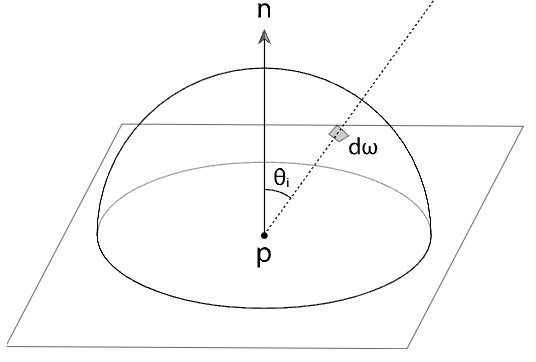
\includegraphics[scale=0.5]{./Imagens/irradiance_hemisphere.png}
        \end{center}
  \legend{ \small Fonte: \cite{pbr}. Adaptada.}
\end{figure}


\begin{figure}[h]
  \caption{\label{solid-angle} \small   Ângulo sólido s do objeto B visto pelo ponto p. }
        \begin{center}
            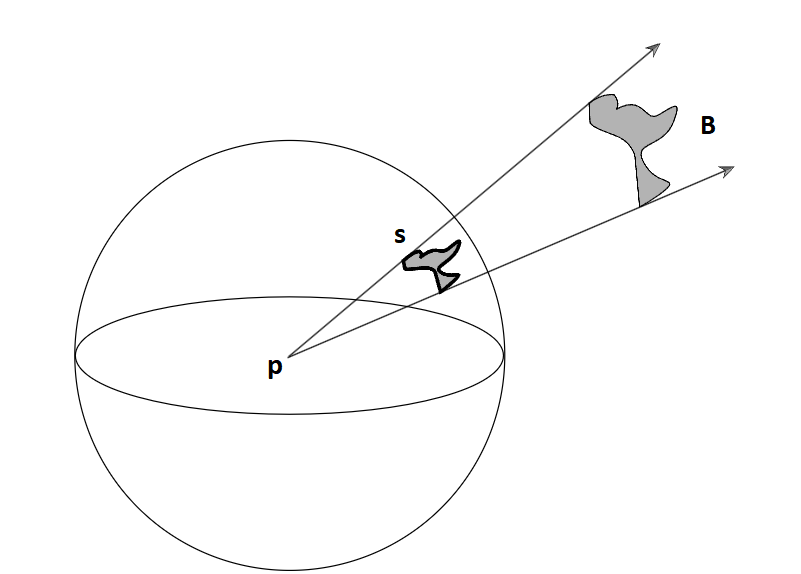
\includegraphics[scale=0.5]{./Imagens/solid_angle.png}
        \end{center}
  \legend{ \small Fonte: \cite{pbr}.}
\end{figure}




% \begin{align*} 
%   L(p,{\omega}) &= \frac{dE_{\omega}(p)}{d{\omega}} \qquad \left[\frac{J}{s\cdot m^2\cdot \text{sr}}\right]\\ 
% E_{\omega} &\text{ é função de irradiância numa direção ${\omega}$ } 
% \end{align*}


Equivalentemente, podemos definir radiância para diferentes orientações da superfície e direção do raio ao introduzir o fator $\cos(\theta)$, tal que $\theta$ é o ângulo entre a normal da superfície e a direção ${\omega}$ \cite[5.4.1]{pbr}. Essa definição é dada pela \autoref{eq-radiance-2}. 


\begin{equation} \label{eq-radiance-2}
  L(p,{\omega}) = \frac{d^2\phi(p)}{dAd{\omega} \cos(\theta)} = \frac{dE(p)}{d{\omega} \cos(\theta)} 
\end{equation}




A radiância pode fornecer informação sobre o quanto um ponto específico está iluminado na direção da câmera. Ela depende não apenas da direção do raio que incide, mas também das propriedades de refletância da superfície. E, no contexto de renderização, a radiância de uma superfície na cena se correlaciona com a irradiância de um pixel em uma imagem pela \autoref{eq-radiance-2}. Isolando o termo $E(p)$, encontramos essa relação de maneira explícita na \autoref{eq-irradiance-explicit}.


\begin{equation} \label{eq-irradiance-explicit}
  \begin{aligned}
  &E(p) = \int_{H^2}{L(p,{\omega})\cos(\theta)d{\omega}}\\
  &H^2 \text{ é o hemisfério no plano tangente à superfície no ponto $p$}
  \end{aligned}
\end{equation}




A principal funcionalidade de um renderizador fotorrealista é estimar a radiância em um ponto $p$ numa dada direção ${\omega}_o$. Essa radiância é dada pela \autoref{eq-rendering-equation}, conhecida como equação de renderização apresentada por \citeonline{rendering_equation}. Note que essa equação envolve um termo de radiância recursivo; o caso base ocorre quando não há mais o termo recursivo, isto é, a radiância é contribuída apenas por radiância emitida $L_e$, como ocorre com fontes de luz.


\begin{equation}\label{eq-rendering-equation}
\begin{aligned}
  &L_o(p, {\omega}_o) = L_e(p, {\omega}_o) + 
\int_{H^2}f(p, {\omega}_i, {\omega}_o){L_i(p,{\omega}_i)\cos(\theta_i)d{\omega}_i}\\
    &L_o \text{ é radiância de saída (\textit{outgoing})}\\
    &L_e \text{ é radiância emitida pela superfície (i.e. fonte de luz)}\\
    &L_i \text{ é radiância incidente na superfície}\\
    &{\omega}_i \text{ é a direção incidente}\\
    &{\omega}_o \text{ é a direção de saída}\\
    &H^2 \text{ são todas as direções no hemisfério no ponto $p$}\\
    &\theta_i \text{ ângulo entre direção incidente e a normal da superfície}\\
    &f \text{ função de refletância}\\
\end{aligned}
\end{equation}


A Função de Distribuição Bidirecional de Reflectância (BRDF) descreve como a luz reflete de uma superfície em diferentes direções, afetando a radiância de saída \cite{overview_brdf}. Assim, BRDFs encapsulam as propriedades de reflexão de um material, considerando fatores como a rugosidade da superfície, o ângulo de incidência e o ângulo de reflexão. Formalmente uma BRDF pode ser definida por $f({\omega}_i, {\omega}_o)$, onde ${\omega}_i$ é a direção incidente de luz e ${\omega}_o$ é a direção de saída. Para BRDFs fisicamente realistas, algumas propriedades devem ser respeitadas \cite[5.6]{pbr}:


\begin{itemize}
  \item A positividade, $f(\omega_i, \omega_o) \geq 0 $, que garante não existência de energia negativa. 


  \item A reciprocidade de Helmhotz, $f(\omega_i, \omega_o) = f(\omega_o, \omega_i)$, é o princípio que indica que a função de refletância de uma superfície permanece inalterada quando os ângulos de incidência e reflexão da luz são trocados. Isso é utilizado na otimização do traçado de raios durante a renderização, permitindo traçar os raios da câmera para a fonte de luz. Essa abordagem evita o desperdício computacional em raios que não contribuem significativamente para a intensidade de um pixel na imagem final.


  \item A conservação de energia, expressa por $\forall \omega_i, \int_{H^2}{f(\omega_i, \omega_o)cos(\theta_o) d\omega_o} \leq 1$, implica que parte da energia pode ser absorvida, transformando-se em outras formas de energia, como calor. Portanto, a soma infinitesimal pode atingir no máximo 1, mas nunca ultrapassá-la.
\end{itemize}


\section{Modelos de BRDFs } \label{brdfmodels}
As próximas seções apresentam alguns modelos comuns de BRDFs  na literatura \cite{overview_brdf}.




\subsection{BRDF Pura Especular}
Uma superfície puramente especular reflete a luz apenas em uma direção, seguindo a lei física da reflexão \cite{laws_of_refletion}, ela produz reflexões nítidas, semelhantes a espelhos. A BRDF para essa superfície é frequentemente representada pela \autoref{eq-specular}, onde $\omega_i$ é a direção da luz incidente, $\omega_o$ é a direção refletida e $\delta$ é a função delta de Dirac que garante que toda a luz incidente seja refletida na direção perfeitamente espelhada como na \autoref{specular}. Esse tipo de superfície é comum em materiais como metal polido ou vidro.


\begin{equation} \label{eq-specular}
f(\omega_i, \omega_o) = k_s \cdot \delta(\omega_i - \omega_o)
\end{equation}


\begin{figure}[H]
        \caption{\label{specular} \small Reflexão especular. Em vermelho está o raio incidente, e em azul o raio de saída.}
        \begin{center}
            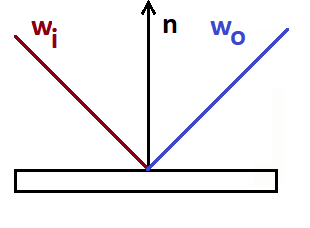
\includegraphics[scale=0.5]{./Imagens/specular-2d.png}
        \end{center}
        \legend{ \footnotesize 
  Fonte: Autor.}
\end{figure}


\subsection{BRDF Difusa Ideal}
Uma BRDF difusa ideal reflete a luz incidente uniformemente em todas as direções, sem preferência por ângulos específicos. É representada pela função $f$ na \autoref{eq-diffuse}, onde $\rho_d$ é o albedo da superfície\footnote{Albedo: propriedade óptica que quantifica a fração da radiação incidente que é refletida por uma superfície. Varia de 0 (superfície totalmente absorvente) a 1 (superfície que reflete toda a luz incidente)} e $\theta$ é o ângulo entre a direção da luz incidente e a normal da superfície. O termo cosseno garante que a radiância refletida seja proporcional ao cosseno do ângulo entre a direção da luz incidente e a normal da superfície, como ilustrado na \autoref{diffuse}. Esse modelo pode representar superfícies como tinta fosca ou papel.


\begin{equation} \label{eq-diffuse}
f(\omega_i, \omega_o) = \frac{\rho_d}{\pi} \cdot \cos \theta
\end{equation}


\begin{figure}[H]
        \caption{\label{diffuse} \small Reflexão Difusa. Note que os raios refletidos não dependem do ângulo de entrada.}
        \begin{center}
            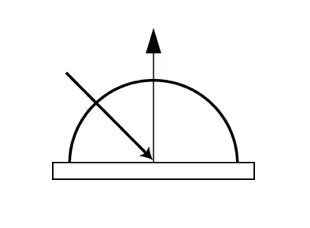
\includegraphics[scale=0.5]{./Imagens/diffuse-2d.png}
        \end{center}
        \legend{ \footnotesize Fonte: Autor. }
\end{figure}


\subsection{BRDF \textit{Glossy}}
Uma superfície pode exibir propriedades de reflexão tanto especulares quanto difusas, como na \autoref{glossy}. Uma BRDF para uma superfície brilhante é frequentemente representada por uma combinação de termos especulares e difusos, como o modelo de Blinn-Phong \cite{blinn_phong}.


\begin{figure}[H]
  \caption{\label{glossy} \small Reflexão \textit{glossy}. }
        \begin{center}
            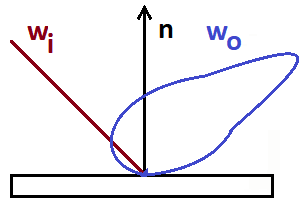
\includegraphics[scale=0.5]{./Imagens/glossy-2d.png}
        \end{center}
        \legend{\footnotesize  Fonte: Autor.}
\end{figure}




\subsection{BRDF Retro-Refletora}
Uma superfície retro-refletora reflete a luz incidente de volta na direção de onde veio, como na \autoref{retro_refletora}. A BRDF para uma superfície retro-refletora envolve tipicamente geometria especializada ou revestimentos projetados para redirecionar a luz de volta para a fonte.


\begin{figure}[H]
  \caption{\label{retro_refletora} \small Reflexão retro-refletora.}
        \begin{center}
            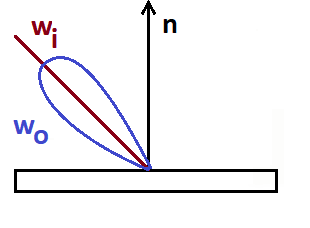
\includegraphics[scale=0.5]{./Imagens/retro-reflection-2d.png}
        \end{center}
        \legend{\footnotesize  Fonte: Autor.}
\end{figure}




\section{Introdução ao Shading e ao \textit{pipeline} de GPU} \label{shading}


\textit{Shading} refere-se ao processo de determinar a cor e o brilho dos pixels em uma imagem renderizada. Isso envolve simular a interação da luz com as superfícies, levando em consideração as propriedades dos materiais, condições de iluminação e orientação da superfície. Isso é alcançado por meio de pequenos programas chamados \textit{shaders}, que são compilados e executados na unidade de processamento gráfico (GPU).




A interação com as GPUs é facilitada por meio de uma 
API, sendo o OpenGL uma API padrão para o uso de funções na GPU \cite{opengl_spec}. O \textit{pipeline} de renderização do OpenGL é composto por várias etapas, incluindo definição de dados de vértices, \textit{shaders} de vértice e fragmento, \textit{shaders} de tesselação e geometria opcionais, configuração de primitivas, recorte e rasterização.


% Essas etapas coordenam o fluxo de dados da CPU para a GPU e suas transformações, culminando na geração da imagem final. As etapas mais importantes para o nosso trabalho são os \textit{shaders} de fragmento e de vértice, representados na \autoref{fig-pipeline}, os quais executam a manipulação dos vértices e determinam cores de pixels, respectivamente.


Essas etapas coordenam o fluxo de dados da CPU para a GPU e suas transformações, culminando na geração da imagem final. Uma representação visual desse processo pode ser observada na \autoref{fig-pipeline}. Nela, é representado a CPU enviando os dados da cena para a GPU, que utiliza essas informações nos \textit{shaders} de vértice e fragmento. O \textit{shader} de vértice manipula os vértices da cena, enquanto o \textit{shader} de fragmento determina as cores dos pixels. Os fragmentos são elementos gerados durante o processamento das primitivas geométricas, como triângulos. Eles correspondem a pontos discretos na tela onde a cor final será determinada. Além disso, a CPU também pode enviar variáveis uniformes (\textit{uniform variables}) para os \textit{shaders}, que são essenciais para a etapa de renderização e contribuem para a geração da imagem final.


\begin{figure}[H]
        \caption{\label{fig-pipeline}\small O \textit{pipeline}.}
        \begin{center}
            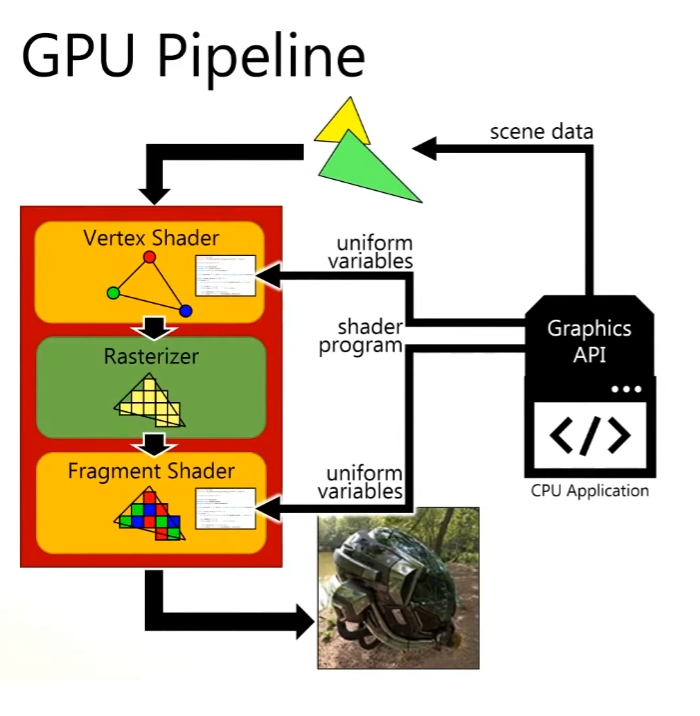
\includegraphics[scale=0.45]{./Imagens/gpu_pipeline.png}
        \end{center}
  \legend{Fonte: \cite{video_pipeline}.}
\end{figure}




\subsection{Shader de Vértice}


O \textit{shader} de vértice opera em vértices individuais de primitivas geométricas antes de serem rasterizados em fragmentos. Sua principal tarefa é transformar vértices e passar os dados necessários para o \textit{shader} de fragmentos. Esses \textit{shaders} geralmente realizam várias transformações nos dados dos vértices, permitindo que objetos sejam posicionados, orientados e projetados em uma tela bidimensional (2D). Um exemplo desse \textit{shader} está no \autoref{vertex_code1}, que usa uma matriz para realizar essas transformações. Ao fim dessa etapa, os vértices são normalizados para coordenadas homogêneas. Essa normalização é essencial para realizar a projeção perspectiva e outros cálculos no \textit{pipeline} de renderização.




\begin{codigo}[H]
  \caption{\small Exemplo GLSL de \textit{shader} de vértice.}
 \label{vertex_code1}
\begin{lstlisting}
#version 330 core
layout(location = 0) in vec3 inPosition;
layout(location = 1) in vec3 inNormal;


uniform mat4 modelViewProjection;


out vec3 fragNormal;


void main() {
    vec3 manipulatedPosition = inPosition + (sin(gl_VertexID * 0.1) * 0.1);
    fragNormal = inNormal;
    gl_Position = modelViewProjection * vec4(manipulatedPosition, 1.0);
}
\end{lstlisting}
\end{codigo}


\subsection{Shader de Fragmento}


O \textit{shader} de fragmento opera sobre os fragmentos produzidos pela etapa de rasterização. Sua principal responsabilidade é determinar a cor final de cada fragmento com base na iluminação, texturização e propriedades da superfície. Uma possível interpretação é que esse programa é repetido para todos os pixels da imagem paralelamente.  Ele recebe dados interpolados, como vértices e normais, ou seja, cada instância desse programa possui entradas potencialmente diferentes uma das outras. Na API OpenGL, valores como normais e vértices são interpolados usando coordenadas baricêntricas \cite{opengl_interpolation}.


As BRDFs podem ser implementadas nesse estágio do \textit{pipeline} para atingir um nível de \textit{shading} mais preciso, pois é possível ter mais dados do que os definidos na geometria devido à interpolação. Isso resulta em um nível de detalhamento potencialmente maior, considerando uma transição mais suave de um ponto para outro dentro de um triângulo,  como representado na \autoref{better-with-fragment}.




\begin{figure}[H]
        \caption{\label{better-with-fragment} \small Diferença entre shading a nível de vértice e shading a nível de fragmento.}
        \begin{center}
            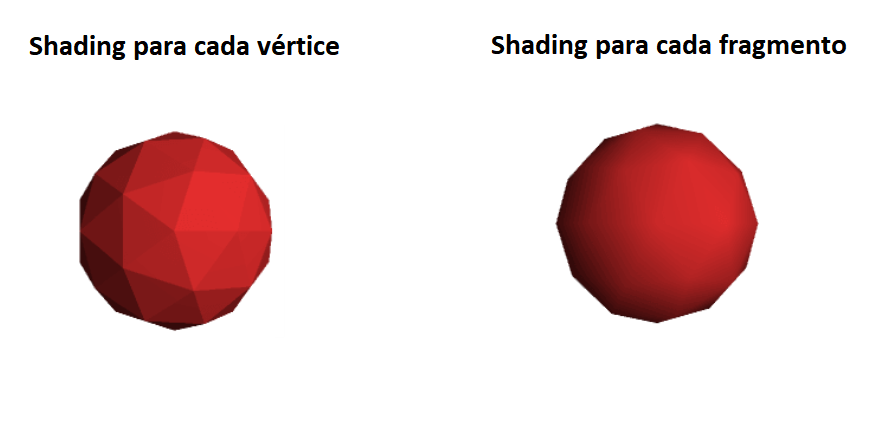
\includegraphics[scale=0.5]{./Imagens/per_vertex_per_frag.png}
        \end{center}
  \legend{ Fonte: \cite{pervertex_perfrag}.}
\end{figure}


\section{Compiladores} \label{compiladores}


\subsection{Cadeia de Símbolos e Alfabeto} \label{símbolos}


Um \textbf{cadeia de símbolos} é uma sequência finita de símbolos retirados de um alfabeto $ \Sigma $. Formalmente, uma cadeia $ w $ é representada como $ [w_1, w_2, ..., w_n] $, onde cada $ w_i $ pertence ao alfabeto $ \Sigma $. O \textbf{alfabeto} $ \Sigma $ é um conjunto finito de símbolos distintos usados para construir cadeias em uma linguagem. Ele define os blocos de construção a partir dos quais cadeias válidas na linguagem são formadas.


\subsection{Definições de Linguagens} \label{linguagem}


Na ciência da computação, as linguagens são sistemas formais compostos por símbolos e regras que são muito úteis para definir um significado algorítmico. Uma \textbf{linguagem} $L$ é definida como um conjunto de cadeias sobre um alfabeto finito $ \Sigma $, $ L \subseteq \Sigma^* $, onde  $ \Sigma^* $ denota o conjunto de todas as cadeias possíveis sobre $ \Sigma $ \cite{language_theory}. A estrutura semântica de uma linguagem inclui seu alfabeto $ \Sigma $, sintaxe e regras de gramática.


\subsection{Compilador como um Transformação}


Um compilador pode ser visto como uma transformação entre linguagens $ L_1 $ e $ L_2 $ que preserva a estrutura interna dos conjuntos, isto é, deve manter o mesmo significado algorítmico. Assim, o compilador $ C: L_1 \rightarrow L_2 $ mapeia programas escritos na linguagem de origem $ L_1 $ para programas equivalentes na linguagem de destino $ L_2 $. Essa transformação garante a preservação semântica, mantendo o comportamento pretendido do programa original durante a tradução.




\subsection{Gramática} \label{gramatica}


Durante a criação de um compilador, é necessário entender as regras que auxiliam na validação da linguagem de entrada, essas regras podem ser formalizadas pela gramática. Uma gramática $G$ é um sistema formal composto por um conjunto de regras de produção que especificam como cadeias válidas na linguagem podem ser geradas \cite{language_theory}. Ela inclui terminais, não-terminais, regras de produção e um símbolo inicial.


\begin{itemize}
  \item Terminais: são os símbolos básicos a partir dos quais as cadeias são formadas. Eles representam as unidades elementares da sintaxe da linguagem.
  \item Não-terminais: são espaços reservados que podem ser substituídos por terminais ou outros não-terminais de acordo com as regras de produção.


  \item Regras de Produção: definem a transformação ou substituição de não-terminais em sequências de terminais e/ou não-terminais.


  \item Símbolo Inicial: é um não-terminal especial a partir do qual a derivação de cadeias válidas na linguagem começa.
\end{itemize}




\subsubsection{Gramáticas Livres de Contexto (GLCs)}


Um tipo comum de gramática usado na definição de linguagens é a gramática livre de contexto (GLC).  Uma GLC pode ser descrita formalmente como $ G=(V,\Sigma,R,S)$:


\begin{itemize}
  \item $V$ é um conjunto finito de símbolos não-terminais.


  \item $\Sigma$ é um conjunto finito de símbolos terminais disjunto de $V$.


  \item $R$ é um conjunto finito de regras de produção, cada regra no formato $A \rightarrow \beta$, onde $A$ é um não-terminal e $\beta$ é uma cadeia de terminais e não-terminais.


  \item $S$ é o símbolo inicial, que pertence a $V$.
\end{itemize}


O processo de gerar uma cadeia na linguagem definida por uma gramática é chamado de derivação. Isso envolve aplicar regras de produção sucessivamente, começando pelo símbolo inicial $S$ até restarem apenas símbolos terminais.


Uma árvore sintática é uma representação gráfica do processo de derivação, onde cada nó representa um símbolo na cadeia. As arestas representam a aplicação de regras de produção. Em código, essa árvore é gerada e usada como representação intermediária,  auxiliando na geração da linguagem alvo $L_2$.




\subsection{Análise Léxica}
A análise léxica, também conhecida como \textit{lexing} ou \textit{tokenization}, é a primeira etapa do processo de compilação, na qual a entrada textual é dividida em unidades léxicas significativas chamadas de \textit{tokens}. Esses \textit{tokens} representam os componentes básicos da linguagem, como palavras-chave, identificadores, operadores e literais. O analisador léxico percorre o código-fonte caractere por caractere, agrupando-os em \textit{tokens} conforme regras pré-definidas pela gramática da linguagem. Essa linguagem é, geralmente, reconhecível por máquinas de estado \cite{automata}.


\subsection{Análise Sintática ou \textit{Parsing}}
A análise sintática é a segunda fase do processo de compilação, na qual os \textit{tokens} gerados pela análise léxica são organizados e verificados quanto à conformidade com a gramática da linguagem. Essa etapa envolve a construção de uma árvore sintática, ou estrutura de dados equivalente, que representa a estrutura hierárquica das expressões e instruções do programa. O analisador sintático utiliza regras de produção gramatical para validar a sintaxe do código-fonte e identificar possíveis erros.


\subsubsection{Pratt Parsing}
O Pratt \textit{Parsing}, introduzido por Vaughan Pratt, é uma técnica de análise sintática recursiva que permite analisar expressões com precedência de operadores de forma eficiente e sem ambiguidades \cite{pratt}. Uma das suas características distintivas é determinar a ordem de avaliação das expressões. Ao contrário da análise descendente recursiva tradicional, na qual cada não-terminal possui uma função de \textit{parsing}, a análise Pratt associa funções de manipulação (\textit{handlers}) com \textit{tokens}.


A precedência das expressões é definida por meio de uma tabela, na qual cada operador é associado a um valor que permita o \textit{parser} decidir dinamicamente a ordem de avaliação das expressões com base nos operadores encontrados durante a análise. Essa abordagem simplifica significativamente a implementação do \textit{parser} e elimina a necessidade de criar uma gramática que encapsula a precedência em sua definição. Ela também evita a recursão profunda para lidar com diferentes níveis de precedência.


% \subsubsection{Árvores Inclinadas}
%
% Em uma árvore inclinada à direita, operadores com maior precedência são resolvidos primeiro, mesmo que apareçam na direita da expressão. Isso resulta em uma árvore onde os operadores com maior precedência estão mais próximos da raiz, indicando que eles são avaliados primeiro. Considere a expressão ``1 + 2 * 3'', apesar de ``*'' aparecer após ``+'',  ``*'' tem uma precedência mais alta e, portanto, forma uma subárvore que é resolvida antes da adição.
%
%
% \begin{verbatim}
%                +
%               / \
%              1   *
%                 / \
%                2   3
% \end{verbatim}
%
% Por outro lado, em uma árvore inclinada à esquerda, operadores com maior precedência são resolvidos por último, seguindo uma ordem de avaliação da esquerda para a direita. As árvores inclinadas à esquerda estão tipicamente associadas a chamadas recursivas de \textit{parsing}, já as inclinadas à direita estão associadas a iteração. Para alcançar a estrutura correta da árvore, o Pratt \textit{parsing} alterna entre recursão e iteração com base na precedência dos operadores para saber o momento de gerar uma subárvore inclinada para esquerda ou direita.


\subsubsection{Pseudo-código para Análise de Expressões}


O pseudo-código \ref{alg1}
demonstra o Pratt \textit{parsing} para a construção de árvores de expressão. Esse algoritmo também é robusto mesmo quando um operador é tanto infixo quanto prefixo, por exemplo ``$-$'' pode ser um \textit{token} de subtração ou de negação. Assim, cada \textit{token} tem uma função de prefixo e infixo associada.


Nesse algoritmo, 
\textbf{proximo\_token()} recupera o próximo elemento da lista de \textit{tokens},
\textbf{token.precedencia}() retorna a procedência do token atual, \textbf{token.prefixo()} é a função associada ao \textit{token} que faz o \textit{parsing} de uma expressão quando o \textit{token} é o primeiro símbolo em uma subexpressão (e.g. o token ``$-$'' é o primeiro na expressão ``$-3$''). Enquanto o \textbf{token.infixo(esquerda)} é a função associada ao \textit{token} que utiliza outra subárvore já criada como entrada. Por exemplo a subárvore \textbf{esquerda} pode ser a expressão ``$-3$'', o \textit{token} atual ser ``$*$'' e o retorno gera a expressão completa ``$-3 * 1$''.


Tanto \textbf{token.infixo} quanto \textbf{token.prefixo} podem ser indiretamente recursivas, isto é, ambas podem chamar a função \textbf{expressão} no \autoref{alg1}. 
Por fim, \textbf{precedencia\_anterior} representa a precedência do \textit{token} anterior.


\begin{algoritmo}[H]
        \caption{\small Função Pratt Parsing de Expressão.}
        \label{alg1}
  \begin{lstlisting}
  function expressao(precedencia_anterior:=0):
      token := proximo_token()
      esquerda := token.prefixo()
      while precedencia_anterior < token.precedencia():
          token    = proximo_token()
          esquerda = token.infixo(esquerda)
      return esquerda
  \end{lstlisting}
\end{algoritmo}


\subsection{Análise Semântica}


A análise semântica é uma etapa essencial no processo de compilação, responsável por garantir a corretude semântica das declarações e instruções do programa. Durante essa fase, são aplicadas verificações para garantir que as operações sejam realizadas com tipos compatíveis.


Um exemplo típico de verificação semântica é a inferência de tipos em expressões. Por exemplo, no \autoref{cod-exemplo-c} o analisador semântico infere que o número inteiro $30$ deve ser convertido para o tipo \textit{float} antes da multiplicação, garantindo consistência de tipos. Além da verificação de tipos, o analisador semântico identifica e reporta outros erros comuns, como variáveis não declaradas e falhas no controle de fluxo do programa.


\begin{codigo}
\caption{\small Exemplo de código escrito em C.}
  \label{cod-exemplo-c}
\begin{lstlisting}[language=C]
float x = 10.1;
float y = x * 30;
\end{lstlisting}
\end{codigo}



No contexto deste trabalho, a análise semântica é importante para validar expressões e funções relacionadas à renderização de materiais no desenvolvimento de \textit{shaders} no OpenGL. Por exemplo, ao escrever uma função BRDF em GLSL, o analisador deve verificar se os tipos de dados e operações são compatíveis tanto com a definição da função BRDF quanto com as dimensões de vetores e outras grandezas definidas.


\subsection{Geração da Linguagem Alvo} \label{codegen}


Nesta fase, fazemos a transição da representação intermediária  da linguagem origem \( L_1 \)  para  a linguagem de destino \( L_2 \), processo que envolve traduzir construções de \( L_1 \) para equivalentes em $L_2$. Podemos realizar essa tradução ao percorrer recursivamente os nós da árvore sintática usando as informações contidas nesses nós para gerar partes do programa final em $L_2$.


Dado um programa $a \in L_1$ existem vários programas $b_{i=1,2,3,...} \in L_2$ que possui estrutura semanticamente equivalentes à $a$. Ao explorar esse conjunto, é possível escolher um $b_j \in L_2$ tal que esse programa seja otimizado em algum sentido, como uso eficiente de memória ou executar menos instruções de \textit{hardware}. Nosso foco neste trabalho está na tradução semanticamente correta, sem envolver exploração das saídas  equivalentes.


Como exemplo, considere a tradução de um cálculo matemático de \( L_1 \) (\LaTeX{}), para \( L_2 \) (GLSL). O cálculo apresentado na \autoref{eq-calculo-vetorial} pertence a $L_1$. O \autoref{cod-fonte-calculo} mostra o código-fonte desse cálculo. 




\begin{equation} \label{eq-calculo-vetorial}
 \quad \mathbf{v} = (\mathbf{a} + \mathbf{b}) \cdot
 \mathbf{c} - (\mathbf{d} \times \mathbf{e})
\end{equation}


\begin{codigo}
  \caption{\small Cálculo vetorial em código-fonte \LaTeX{}.}
  \label{cod-fonte-calculo}
\begin{lstlisting}
 \mathbf{v} = (\mathbf{a} + \mathbf{b}) \cdot
 \mathbf{c} - (\mathbf{d} \times \mathbf{e})
\end{lstlisting}
\end{codigo}






Após a tradução da expressão matemática para \( L_2 \), o cálculo pode ser convertido para o trecho de programa apresentado no \autoref{cod-calculo-vetorial-glsl}. Esse código é válido na linguagem GLSL.


\begin{codigo}
\caption{\small Cálculo vetorial em código GLSL.}
\label{cod-calculo-vetorial-glsl}
\begin{lstlisting}[language = C]
    vec3 v = dot(a + b, c) - cross(d, e);
\end{lstlisting}
\end{codigo}



